\documentclass[two column]{article}
\usepackage[utf8]{inputenc}
\usepackage{amssymb}
\usepackage{indentfirst}
\usepackage{tikz}
\usetikzlibrary{shapes.geometric, arrows}
\setlength{\parindent}{2em}
\usepackage{url}
\usepackage{booktabs}
\usepackage[colorlinks=false]{hyperref}
\usepackage{listings}
\usepackage{graphicx}
\graphicspath{ {./images/} }
\usepackage{caption}
\usepackage{natbib}
\usepackage{graphicx}
\usepackage{float} %设置图片浮动位置的宏包
\usepackage{stfloats}
\lstset{
  basicstyle=\ttfamily,
  columns=fullflexible,
  breaklines=true,
  aboveskip=26pt,belowskip=0pt
}

\newenvironment{figurehere}
{\def\@captype{figure}}
{}
\newcommand{\beq}{\begin{equation}}
\newcommand{\bseqs}{\begin{subequations}}
\newcommand{\eseqs}{\end{subequations}}
\newcommand{\balign}{\begin{align}}
\newcommand{\ealign}{\end{align}}
\newcommand{\eeq}{\end{equation}}
%\newcommand{\beq}{\begin{eqnarray*}}
%\newcommand{\eeq}{\end{eqnarray*}}
\newcommand{\beql}{\begin{equation} \label}
\newcommand{\beqs}{\begin{eqnarray}}
\newcommand{\eeqs}{\end{eqnarray}}
\newcommand{\beas}{\begin{eqnarray*}}
\newcommand{\eeas}{\end{eqnarray*}}
\newcommand{\ber}{\begin{array}}
\newcommand{\eer}{\end{array}}
\newcommand{\becs}{\begin{cases}}
\newcommand{\eecs}{\end{cases}}

\title{Movie Recommendation system }
\author{Group 26 Yan Gu, Xinyang Wang }
\date{Oct 23, 2019 }

\begin{document}
\maketitle
\section{Project Proposal}
\subsection{General system description}
Movie recommendation systems are movie information filtering system that help recommend movies that users are likely interested in. This technology is widely used in today's online e-commerce websites like Amazon, Tmall and so on. There are many techniques that can be used to build such a system. And in this project, we plan to build a simple movie recommendation system model and by using this model, we can generate movies for our users.


\subsection{Project Time line}
\subsubsection{Date:09/04--09/25}
\par Search for topics that we are interested in and decide which topic to choose;
\par ~

\par Search for some documents and thesis and have a basic understanding of what techniques we are going to use.

\subsubsection{Date:09/26--10/16}
\par Choose the data we are going to work on from open source data base, describe the data format and data processing flow.
\par ~

\par Describe the data content using spark.
\par ~

\par Describe the next step that we will proceed with on processed data.
\par ~

\subsubsection{Date:10/17--12/14}
\par Achieve a simple movie recommendation system model. Use this model to do some tests to verify the capacity of our model and evaluate the results numerically or via visualizations.
\par ~

\par Write the final report.


\section{Data Source $\&$ Format $\&$ Preprocessing}
\subsection{Data source}
\par The data we use to do experiments and to draw conclusion from in this project is MovieLens 1M Dataset (link: https://grouplens.org/datasets/movielens/), which contains 1 million ratings from 6000 users on 4000 movies(Released 2/2003). It is from MovieLens data sets, which are collected and made available from MovieLens web site (link: http://movielens.org) by GroupLens Research. MovieLens data sets are the most popular sets used for relevant scientific researches for their accuracy and authenticity.

\subsection{Data Format}
\par MovieLens 1M Dataset contains three major files, which are movies.dat, ratings.dat and users.dat. Below we will show the data format of each file.

\begin{itemize}
\item[1] movies.dat
\par Movie information is in the file "movies.dat" and is in the following format:
\par MovieID::Title::Genres

\par Below is a screenshot of the data for clearer illustration:
\begin{figure}[H]
\centering
\caption{data in movies.dat}
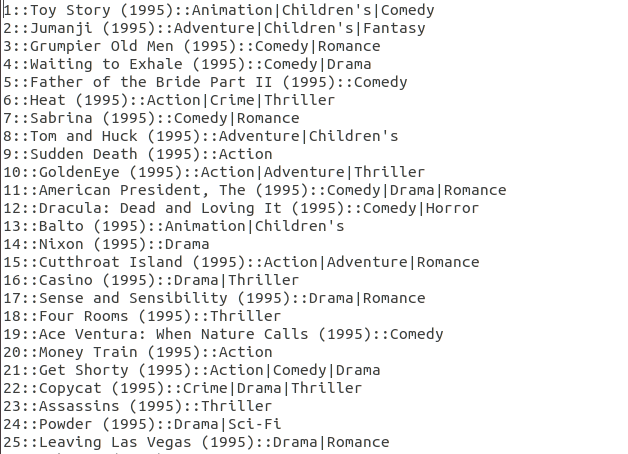
\includegraphics[width = 0.95\linewidth]{p1.png}
\end{figure}

\par Some further explanations below:
\begin{itemize}
\item[(1)] Titles are identical to titles provided by the IMDB (including year of release)

\item[(2)] Genres are pipe-separated and are selected from the following genres:
\par * Action
	* Adventure
	* Animation
	* Children's
	* Comedy
	* Crime
	* Documentary
	* Drama
	* Fantasy
	* Film-Noir
	* Horror
	* Musical
	* Mystery
	* Romance
	* Sci-Fi
	* Thriller
	* War
	* Western
\end{itemize}


\item[2] ratings.dat
\par All ratings are contained in the file "ratings.dat" and are in the following format:
\par UserID::MovieID::Rating::Timestamp

\par Below is a screenshot of the data for clearer illustration:
\begin{figure}[H]
\centering
\caption{data in ratings.dat}
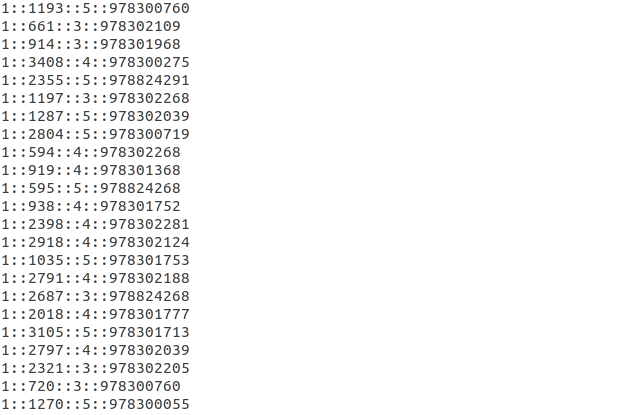
\includegraphics[width = 0.95\linewidth]{p2.png}
\end{figure}

\par Some further explanation:
\begin{itemize}
\item[(1)] UserIDs range between 1 and 6040 
\item[(2)] MovieIDs range between 1 and 3952
\item[(3)] Ratings are made on a 5-star scale (whole-star ratings only)
\item[(4)] Timestamp is represented in seconds since the epoch as returned by time(2)
\end{itemize}

\item[3] users.dat
\par User information is in the file "users.dat" and is in the following format:
\par UserID::Gender::Age::Occupation::Zip-code

\par Below is a screenshot of the data for clearer illustration:
\begin{figure}[H]
\centering
\caption{data in users.dat}
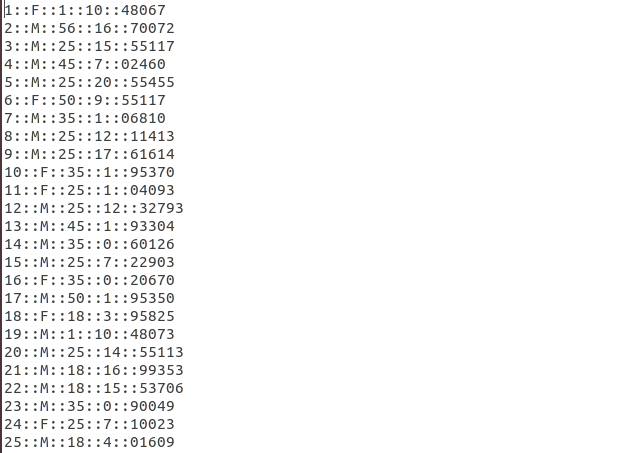
\includegraphics[width = 0.95\linewidth]{p3.png}
\end{figure}

\par Some further explanation:
\begin{itemize}
\item[(1)] Gender is denoted by a "M" for male and "F" for female
\item[(2)] Age is chosen from the following ranges: 
	*  1:  "Under 18"
	* 18:  "18-24"
	* 25:  "25-34"
	* 35:  "35-44"
	* 45:  "45-49"
	* 50:  "50-55"
	* 56:  "56+"
\item[(3)] ccupation is chosen from the following choices:
	*  0:  "other" or not specified
	*  1:  "academic/educator"
	*  2:  "artist"
	*  3:  "clerical/admin"
	*  4:  "college/grad student"
	*  5:  "customer service"
	*  6:  "doctor/health care"
	*  7:  "executive/managerial"
	*  8:  "farmer"
	*  9:  "homemaker"
	* 10:  "K-12 student"
	* 11:  "lawyer"
	* 12:  "programmer"
	* 13:  "retired"
	* 14:  "sales/marketing"
	* 15:  "scientist"
	* 16:  "self-employed"
	* 17:  "technician/engineer"
	* 18:  "tradesman/craftsman"
	* 19:  "unemployed"
	* 20:  "writer"
\end{itemize}

\end{itemize}

\subsection{Data preprocessing}
\par The data stored in the "*.dat" is a number of rows of byte string and the data in the "*.csv" is a Dataframe with column indices. Since the data structure used in the Spark is Dataframe, in order to simplify the data analysis process when exploring the data, we choose to transfer the raw byte data in "*.dat" to data form stored in the "*.csv" files and replace the tags of occupations and ages with their corresponding name of occupation or range of ages.
\par First, for each row of bytes string, we decode them to be char string and then split the string to columns. For example, for each row in "ratings.dat", we use "::" as separator and transfer the string to a list with format "list([userid, movieid, rating, timestamp])".
\par Then, the next step is to use a map to replace the tags of occupations and ages in the Dataframe with their corresponding values such as "writer", "56+" and so on.
\par After all that have been done, the final step is to output the Dataframe to a csv file and add the column indices which specify the labels of each column. Then, the well defined Dataframe object is ready to be used in the next steps.


\section{Data content}
\par All the data in above three data files are discrete and scattered, we can not draw patterns from them. So this is where spark comes into pictures. By using spark, we can simply and quickly get many interesting result. Below we will show the experiments result we harvest from the raw data.

\begin{itemize}
\item[(1)] number of movies of each genre + average ratings for each genre

\begin{figure}[H]
\centering
\caption{number of movies of each genre}
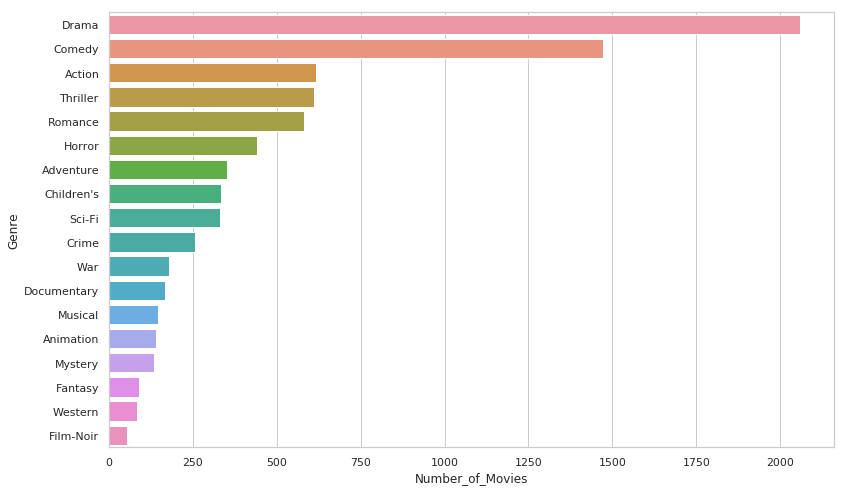
\includegraphics[width = 0.95\linewidth]{numbers-according-to-genre2.png}
\end{figure}

\begin{figure}[H]
\centering
\caption{average ratings for each genre}
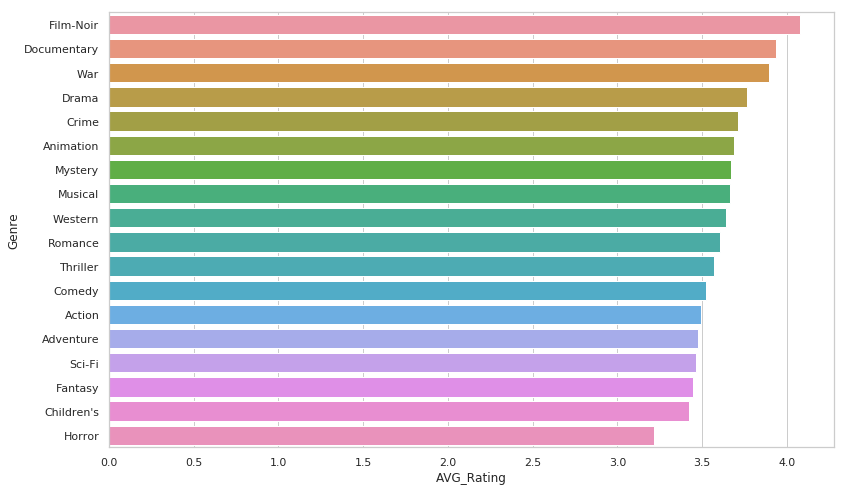
\includegraphics[width = 0.95\linewidth]{ave-ratings-according-to-genre2.png}
\end{figure}

\par We can find out some interesting results from above two figures. For example, Film-Noir is the least popular, but its average rating is the highest. This is reasonable in fact. Because Film-Noir is not popular, people who watch them must be fond of this type, therefore they are very likely to give high ratings.


\item[(2)] average number of rated movies according to career + average rating according to career

\begin{figure}[H]
\centering
\caption{average number of rated movies according to career}
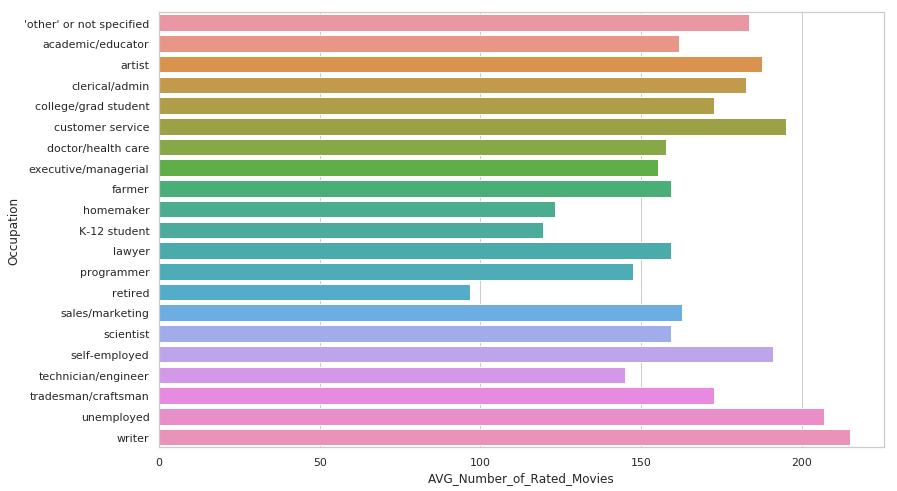
\includegraphics[width = 0.95\linewidth]{career-dis-ave-rated-number-and-ave-rating2.png}
\end{figure}

\begin{figure}[H]
\centering
\caption{average rating according to career}
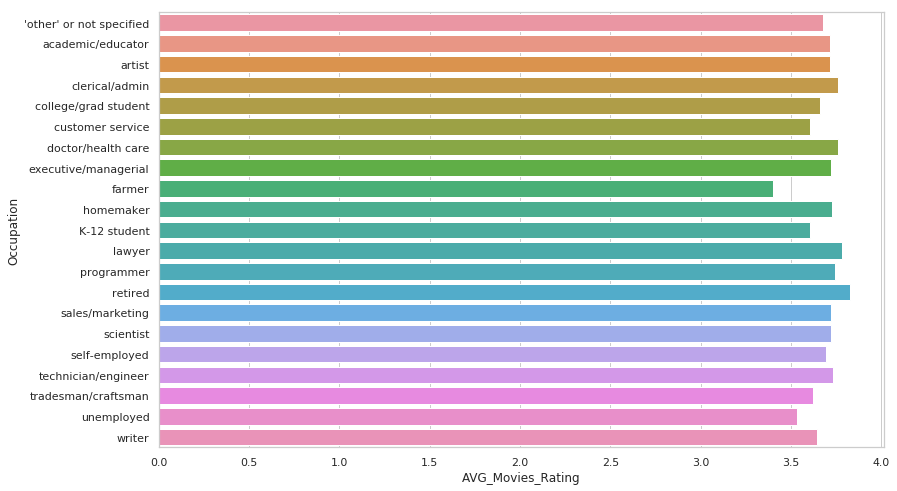
\includegraphics[width = 0.95\linewidth]{career-dis-ave-rated-number-and-ave-rating3.png}
\end{figure}

\par From above, we can also draw some reasonable results. From the first chart, we can see that writers watch the most movies. That may be because they watch movies to get inspiration on their writings. Also unemployed people watch a lot of movie because they got lots of time to consume. 
\par From the second chart, we can see retired people tend to give high ranks. That also comply with reality. elder people are mostly tolerant, even of a bad movie.


\item[(3)] average number of rated movies according to age distribution + average rating according to age distribution

\begin{figure}[H]
\centering
\caption{average number of rated movies according to age distribution}
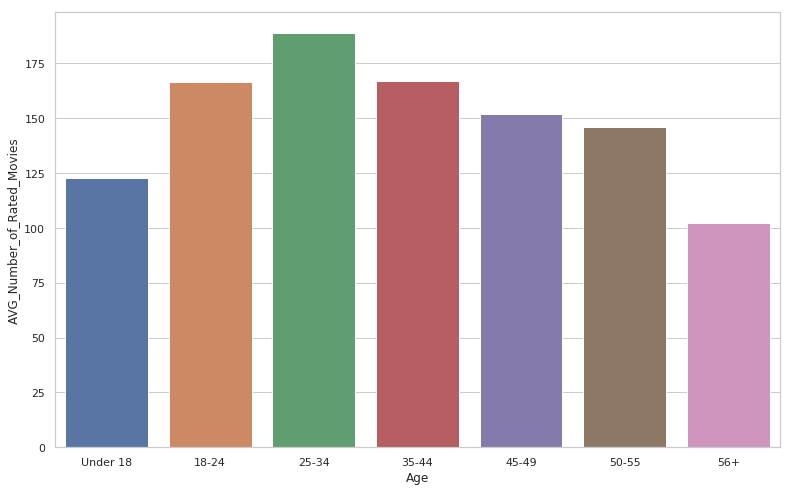
\includegraphics[width = 0.95\linewidth]{age-dis-ave-rated-number-and-ave-rating2.png}
\end{figure}

\begin{figure}[H]
\centering
\caption{average rating according to age distribution}
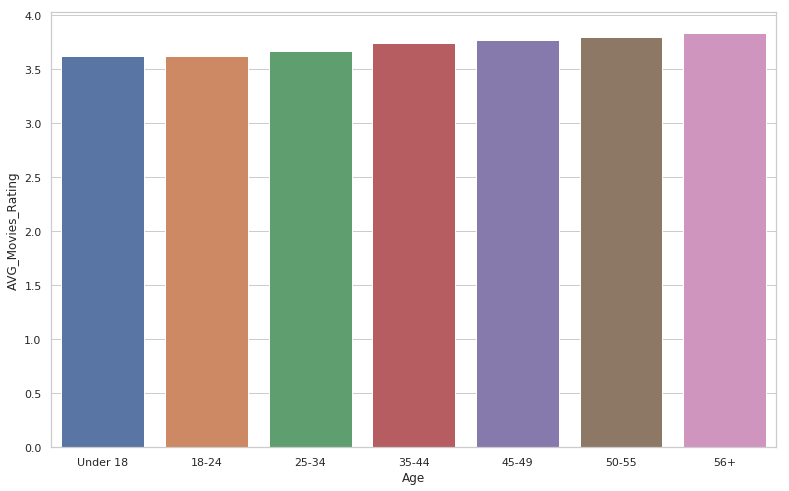
\includegraphics[width = 0.95\linewidth]{age-dis-ave-rated-number-and-ave-rating3.png}
\end{figure}

\par As we can see, people in age span 25-34 watch the most movies, while the number of movies rated decreases as the age of people increases. That is because older people are not as interested as younger people in fashion staff like movies. \par And we can also find out older people gives higher ratings. This result complies with the result in the section above, where we get the result that retired people gives the highest ratings(reired people are usually older people).


\item[(4)] Number of People for each occupation

\begin{figure}[H]
\centering
\caption{Number of People for each occupation}
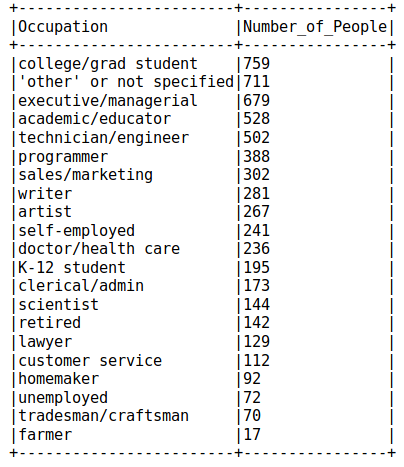
\includegraphics[width = 0.95\linewidth]{career-distribution1.png}
\end{figure}

\par To make it more intuitive, we draw it into a graph.
\begin{figure}[H]
\centering
\caption{Number of People for each occupation}
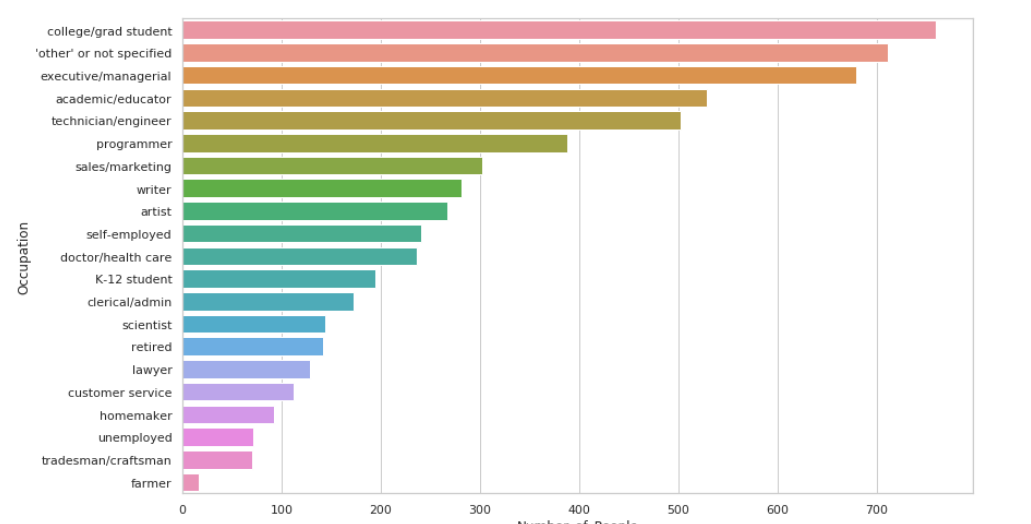
\includegraphics[width = 0.95\linewidth]{career-distribution2.png}
\end{figure}

\par From the figure above, we can find out students are more engaged in this data collection while farmers are less engaged in, which are also comply with our expectation.


\item[(5)] Number of People for each age span

\begin{figure}[H]
\centering
\caption{Number of People for each age span}
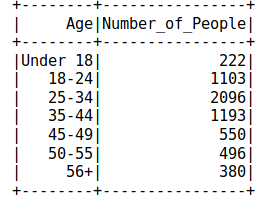
\includegraphics[width = 0.95\linewidth]{age-distribution1.png}
\end{figure}

\par To make it more intuitive, we draw it into a graph.
\begin{figure}[H]
\centering
\caption{Number of People for each age span}
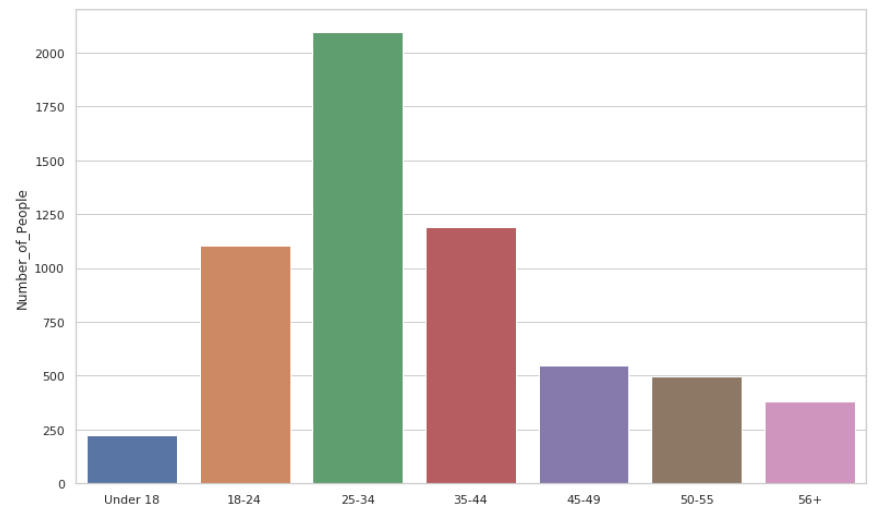
\includegraphics[width = 0.95\linewidth]{age-distribution2.png}
\end{figure}

\par With the chart above, we can find out as the age increases, more people are engaged in data collection, reaching peak at 25-34. And then fewer people engaged in as age increases.

\end{itemize}


\section{Possible Usage of Data}
\par From the results we gain from the data, we might use these results as instructions when doing data collection. For example, we should pay more attention to younger and older people to get more data from them, so that we can get more balanced data.

\par Also because we got ratings in this data, we can try to design a real time movie recommendation system. When people type in the movie they watched with ratings, the system can give out the movies they might be interested in and expected ratings for people to choose from.


\section{Collaborative Filtering}
\par Like many other machine learning techniques, Collaborative Filtering makes prediction based on users' historical behaviors.  Specifically, it’s to predict user preference for a set of items based on past experience. To build a recommendation system using collaborative filtering, there are two approaches that are the most popular: user-based collaborative filtering and item-based collaborative filtering.

\par Let's first look at user-based collaborative filtering. The basic idea is to use the similarity between two different users.
for example, we have an n*m matrix of ratings, with users $u_i$,i=1...n and movies $u_j$,j=1...m. Now if user i does not rate movie j, how do we calculate the expectation of rating $r_{i,j}$ ?
The process is to calculate the similarities between target user i and all other users, select the top K similar users, and take the weighted average of ratings from these K users with similarities as weights.

\par Then let's go to item based collaborative filtering. Instead of computing the similarity between different users, we need to compute the similarity between different items. Suppose we also have the n*m matrix of ratings. Now if movie j is not rated by user i, how do we compute the expectation of rating $r_{i,j}$ ? The process is to calculate the similarities between target movie j and all other movies, select the top K similar movies, and take the weighted average of ratings from these K movies with similarities as weights.

\par While both user-based collaborative filtering and item-based collaborative filtering are powerful in building recommendation system and the computing process is similar, there are some essential differences lying in between. Below we will explain the differences in detail.

\par Firstly, the core of collaborative filtering is to compute the similarity matrix. In user-based collaborative filtering, when a new user comes into the recommendation system, we need to recompute the whole similarity matrix. The recommendation usually contains hundreds of thousands of users and movies. The computation of the similarity matrix is a time-consuming job. So the user-based collaborative filtering could not be used for real-time system.

\par Secondly, user-based collaborative filtering recommend movies according to similar users. While similar users may watch different genres, thus the recommendation result may go out of expectation. As to item-based collaborative filtering, the recommendation results are usually in same genre.

\par Due to the above reasons, we choose item-based collaborative filtering to build the recommendation system.

\section{Flow diagram description}
\par The flow diagram is shown as below, the point is database will be divided into Train data set and Test data set. Train data set will be used to compute movie similarity for every two movies/users and then get the similarity matrix in case of collaborative filtering.

\begin{figure}[H]
\centering
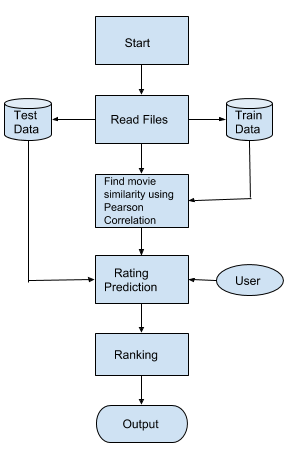
\includegraphics[width=0.5\textwidth]{Flow-chart.png}
\end{figure}


\section{High Level Pseudo Code}
According to flow diagram, there will be three basic steps to get final recommended movies. Firstly, reading data into memory; then, calculating the similarity matrix using cosine or Pearson correlation; Lastly, getting recommended movies according to rating expectation.

\begin{lstlisting}[title=Flow1: Reading file into program, frame=shadowbox]
set up two empty dictionary classes:  
  TrainData={} and TestData={};
for each row in dataset:
  set up a random number used as possibility;
  according to the random number,choose a dictionary to put the value of this row in it
  split the row into for part namely UserID, MovieID, Rating and Timestamp;
  using UserID and MovieID as two keys, and put the ratings according to keys;
\end{lstlisting}
\begin{lstlisting}[title=Flow2: calculate the similarity matrix , frame=shadowbox]
set up distance dictionary:Movie_Dis = {};
set up similarity matrix: Movie_sim = [];
for UserID in TrainData,
  calculate average ratings from each user Ru;
for UserID in TrainData,
  for m1 in TrainData[UserID],
    for m2 TrainData[UserID],
      if m1 != m2
	    calculate the production of distance and put it in Movie_Dis [m1][m2];
for i to number of movies,
  for j to number of movies,
  using Movie_Dis to compute similarity of Movie_sim[i,j] (Pearson coefficient)
\end{lstlisting} 

\begin{lstlisting}[title=Flow3: recommend movies, frame=shadowbox]
given a user's data, traverse the movies he watched;
for each movie he watched,
  compute the expected rating of K(set by us) similar movie;
sort all similar movies and recommend the first L(set by us) movies;
\end{lstlisting}


\section{Time and space complexity description}
\par let's say we have n UserID, and m MovieID, the using of dictionary class decreases the indexing time from O(n)(using list) to O(1), so the we only need to pay attention to 'for' loops. And during the step from 'reading file' to 'recommend movies', the time complexity is O(n$m^2$).

\par The biggest occupation of space lies in generating similarity matrix, which is O(mn).


\section{Experiments results}
\par In our experiments, we design two kinds of input:
\par--users in datasets
\par--new users with historical movies and ratings
\par ~

\par Below are some screenshots of our experimental results. First let's see the recommendation results for users in datasets. We take user with userID 1 as an example. Because we use the user in datasets, we do not need to offer historical movies and ratings. So we just skip the 'input the movies you once watched and ratings' part and directly get the recommendation results as follows.

\begin{figure}[H]
\centering
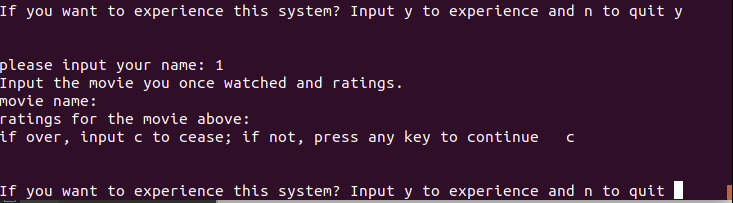
\includegraphics[width=0.5\textwidth]{user-in-dataset.png}
\end{figure}

\begin{figure}[H]
\centering
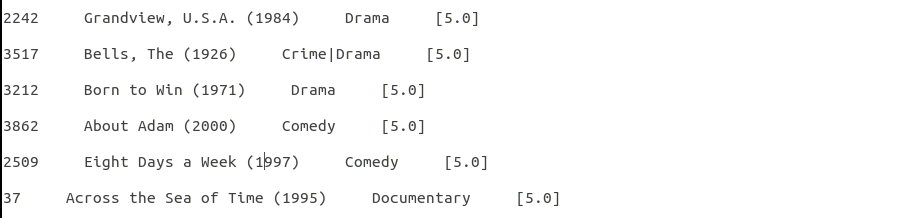
\includegraphics[width=0.5\textwidth]{user-in-dataset1.png}
\end{figure}


\par Then let's see recommendation results for new users. In this part, we need to fill out the movies and the ratings part. We choose the following movies and ratings:
\par 86::White Squall (1996)::Adventure|Drama     rating:5
\par 590::Dances with Wolves (1990)::Adventure|Drama|Western     rating: 3
\par 3004::Bachelor, The (1999)::Comedy|Romance     rating:2
\par ~

\par The results are shown as below and comply with our expectation. In the inputs, we give 5 star rating to movie White Squall (1996), which belongs to adventure and drama. So we can expect that the recommendation system tends to give out movies of genre of adventure or drama. And as we can see, most of the recommendation results belong to drama genre.

\begin{figure}[H]
\centering
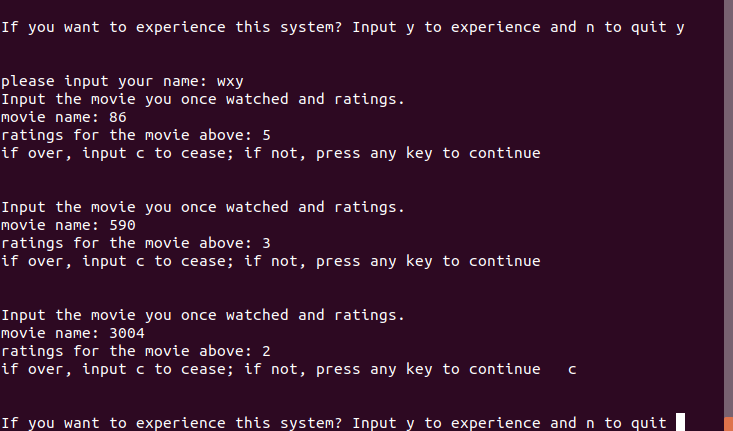
\includegraphics[width=0.5\textwidth]{new-user.png}
\end{figure}

\begin{figure}[H]
\centering
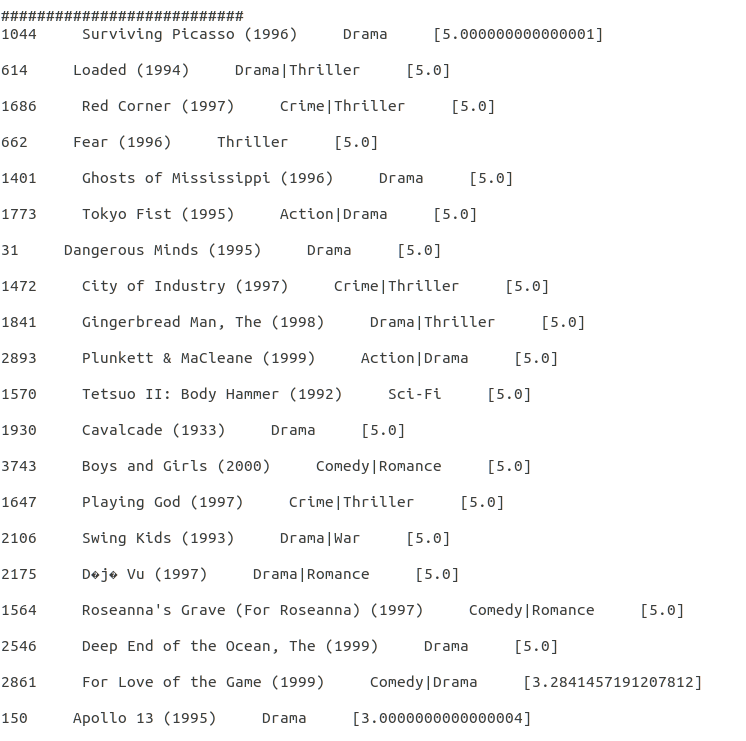
\includegraphics[width=0.5\textwidth]{new-user1.png}
\end{figure}


\section{Conclusion}
\par In this report, we have used spark to analyze the original data and visualize the results in the first half part. In the second half part, we implement item-based collaborative filtering to achieve real-time movie recommendation (after computing the similarity matrix once). Item- based collaborative filtering is powerful and efficient in recommending movies, while there is still room for improvement. For example, using SVD algorithm to reduce the calculation in computing the similarity matrix. 

\end{document}
